\section{Formalization}
\label{sec:formalization}
Given a state space $U$, a transition system $(I,T)$ consists of an
initial state predicate $I : U \to \bool$ and a transition step
predicate $T : U \times U \to \bool$.
We define the notion of
reachability for $(I, T)$ as the smallest predicate $\reach : U \to
\bool$ which satisfies the following formulas:
\begin{gather*}
  \forall u.~ I(u) \Rightarrow \reach(u) \\
  \forall u, u'.~ \reach(u) \land T(u, u') \Rightarrow \reach(u')
\end{gather*}
A safety property $P : U \to \bool$ is a state predicate. A safety
property $P$ holds on a transition system $(I, T)$ if it holds on all
reachable states, i.e., $\forall u.~ \reach(u) \Rightarrow P(u)$,
written as $\reach \Rightarrow P$ for short. When this is the case, we
write $(I, T)\vdash P$. We assume the transition relation has the structure of a top level conjunction. Given $T(u, u') = T_1(u,u') \land \cdots T_n(u,u')$ we will write $T = \land_{i=1..n}T_i$ for short. By further abuse of notation, $T$ is identified with the set of its top-level conjuncts $\land_{i=1..n}T_i$.%\footnote{Each conjunct $T_i$ may contain its own conjuncts; thus, we differentiate by using the term ``top-level" conjunct for the conjunct $T_i$ in the formula $T$.}. 
Thus, $T_i \in T$ means that $T_i$ is a top-level conjunct of $T$, and $S\subseteq T$ means all top level conjuncts of $S$ are top-level conjuncts of $T$. %When a top-level conjunct $T_i$ is removed from $T$, we write $T \setminus \{T_i\}$

The set of all nominal guarantees of the system $G$ consists of conjunctive constraints $g \in G$. Given no faults (i.e., nominal system) and a transition relation $T$ consisting of conjunctive constraints $T_i$, each $g$ is one of the transition constraints $T_i$ where:

\begin{gather}
T = g_1 \land  g_2 \land \cdots \land g_n
\label{eq:Tn}
\end{gather}

We consider an arbitrary layer of analysis of the architecture and assume the property holds of the nominal relation $(I,T) \vdash P$. Let the set of all faults in the system be  denoted as $F$. A fault $f \in F$ is a modification of the nominal constraint imposed by a guarantee. Without loss of generality, we associate a single fault and an associated fault probability with a guarantee. Each fault $f_i$ is associated with an \emph{activation literal}, $\mathit{af_i}$, that determines whether the fault is active or inactive. %Any ``faults" in a mid-layer are simply violated guarantees, or deviations from normal behavior. 

%The faults in the safety annex are defined on leaf level components. Thus, for the lowest analysis layer, we must take into consideration faults and the guarantees their activation may violate. A fault $f \in F$ is a deviation from the normal constraint imposed by a guarantee. For the purposes of this paper, each guarantee at the leaf layer of analysis has an associated fault. 

We extend the transition system so that we can view the system behavior in the presence of faults---or equivalently the absence of nominal constraints. To consider the system under the presence of faults, consider a set $GF$ of modified guarantees in the presence of faults and let a mapping be defined from activation literals $\mathit{af_i} \in AF$ to these modified guarantees $\mathit{gf_i} \in GF$. 
\begin{center}
$\mathit{gf_i} =$ \textit{if} $\mathit{af_i}$ \textit{then} $f_i$ \textit{else} $g_i$
\label{eq:sigma}
\end{center}

The transition system is composed of the set of modified guarantees $GF$ and a set of conjunctions assigning each of the activation literals $\mathit{af_i} \in AF$ to false: 

\begin{gather}
T' = \mathit{gf_1} \land \mathit{gf_2} \land \cdots \land \mathit{gf_n} \land \neg \mathit{af_1} \land \neg \mathit{af_2} \land \cdots \land \neg \mathit{af_n}
\label{eq:T}
\end{gather}

\begin{theorem} If $(I,T) \vdash P$ for $T$ defined in equation~\ref{eq:Tn}, then $(I,T') \vdash P$ for $T'$ defined in equation~\ref{eq:T}.
\begin{proof}
By the mapping of each constrained activation literal $\neg \mathit{af_i}$ to the associated guarantee $g_i$ and the constraint of the activation literals to be false, the result is immediate.
\end{proof}
\end{theorem}

Consider the elements of $T'$ as a set $GF \cup AF$, where $GF$ are the potentially faulty guarantees and $AF$ consists of the activation literals that determine whether a guarantee is faulty. This is a set that is considered by an SMT solver for satisfiability during the model checking engine procedures. 

If the $\mathit{af_i} \in \mathit{AF}$ defined in $T'$ are unconstrained, this allows more behaviors to the transition system and could cause a violation of $P$. If so, a counterexample may be produced. For each counterexample, we can partition $\mathit{AF}$ into two sets that we call {\em non-faulty variables (NFV)} and {\em faulty variables (FV)}.  The set $\mathit{NFV}$ consists of a set of activation literals that are constrained to be false throughout the counterexample, and $\mathit{FV}$ contains those that can be non-deterministically assigned any valuation at some point in the trace. By mapping some of the variables in $\mathit{AF}$ to false, we know that their associated guarantees in $\mathit{GF}$ are non-faulty for all considered executions. We define $T'(\mathit{NFV})$ as a relaxation of $T'$ (\ref{eq:T}):

\begin{gather*}
T'(\mathit{NFV}) = \mathit{gf_1} \land \mathit{gf_2} \land \cdots \land \mathit{gf_n} \land \bigwedge \{\neg \mathit{af_i} | \mathit{af_i} \in \mathit{NFV} \}
\end{gather*}

The activation literals constrained to be false in $T'(\mathit{NFV})$ indicate that their associated guarantees to be valid. In the remainder of this section, we assume that all $\mathit{af_i} \in \mathit{AF}$ are unconstrained and when given a true valuation will lead to a violation of the associated guarantee. This violation causes the output that the guarantee constrains to become non-deterministic. The Boolean variables in $\mathit{FV}$ correspond to Boolean variables in the fault tree. 

%Given the extended transition system in Equation~\ref{eq:T}, if the $\mathit{af_i} \in \mathit{AF}$ are unconstrained and this causes violation of $P$, a counterexample is returned.  This counterexample is a partition of guarantees $\mathit{GF}$ into disjoint sets:  $\mathit{GF} = \mathit{NFV} \cup \mathit{FV}$. The set $\mathit{NFV}$ consists of nonfaulty variables: the associated $\mathit{af_i}$ are mapped to {\em false} in the counterexample, and the set $\mathit{FV}$ consists of faulty variables: the associated $\mathit{af_i}$ are mapped to {\em true} in the counterexample. In the remainder of this section, we assume that all $\mathit{af_i} \in \mathit{AF}$ are nondeterministically unconstrained and when active, cause the associated guarantee to be violated. Thus the output that the guarantee constrains becomes nondeterministic when the associated $\mathit{af_i}$ is true.


%%						DEFINE FT/FF
\begin{definition}
A fault tree $\mathit{FT}$ is a pair $(r, \mathcal{L})$ where:
\begin{itemize}
\item[] $r$: the root $r$ is a negated desirable property
\item[] $\mathcal{L}$: a Boolean equation whose literals are faulty variables
\end{itemize}
%The fault tree $\mathit{FT}$ is a Boolean equation in disjunctive normal form (DNF): $(r, \mathcal{L}) = r \lor \mathcal{L} = r \lor C_1 \lor \cdots \lor C_n$ for conjunctions $C_i$. 
\end{definition}

All literals $\mathit{af}$ of the Boolean equation $\mathcal{L}$ are elements of the set $\mathit{FV}$. A fault tree may correspond to a single layer of the system architecture where the root $r$ is a violated guarantee or a violated safety property depending on the parent component under analysis. The tree may also describe the relationship between faults and multiple layers of the system architecture. The root $r$ still corresponds to a violated guarantee or property, but the structure of the Boolean formula $\mathcal{L}$ will reflect the layers of the system architecture. If $r$ is a violated safety property, then $r \in P$. If $r$ is a violated guarantee for some lower level parent component, then $r \in \pi$, where $\pi$ is the set of parent component guarantees. 

\begin{definition} 
A fault tree $FT = (r, \mathcal{L})$ is valid if and only if a true valuation for $r$ and for all $\mathit{af} \in \mathcal{L}$ is satisfiable given the respective transition system constraints. 
\label{def:validFT}
\end{definition}

The hierarchy of the fault tree is dependent on the associated Boolean formula. A more intuitive structure is that of {\em disjunctive normal form} (DNF) as seen in both fault trees depicted in Figure~\ref{fig:sensorSysComp}, but DNF is not required under our definition of a fault tree. 

Traditionally, a safety property is a property of the system and in the assume-guarantee reasoning environment is a top level guarantee. In the following formalism, each layer of analysis is viewed as distinct from the system hierarchy as the proof is being constructed, and the properties we wish to prove are guarantees of a component. We use the notation $P$ to refer to the set of all parent properties at a given layer of analysis. If the analysis is being performed at the top level, these are all safety properties of the system. If the analysis is being performed at an intermediate level, these are all guarantees of the parent component.

A goal of compositional safety analysis is to reflect failures of leaf and intermediate components at the top level. Not all guarantees must be valid to prove a parent level guarantee. To this end, we wish to make a distinction between all guarantees of a component and those that are required to prove parent guarantees. The subset $\pi$ of $P$ are the guarantees that must be valid to prove the guarantees of a parent component. These are the critical guarantees of a component.

Given that there may be multiple safety properties and multiple intermediate level guarantees, we do not compose single fault trees per layer, but rather forests of trees.

\begin{definition}
A fault forest $\mathit{FF}$ is a set of fault trees.
\end{definition}

\begin{definition}
A fault forest $\mathit{FF}$ is valid if and only if for all $ \mathit{FT} \in \mathit{FF}$, the fault tree $\mathit{FT}$ is valid as per Definition~\ref{def:validFT}.
\label{def:validFF}
\end{definition}

The goal of this formalization is to show that the composition of fault forests results in a valid fault forest. First, we assume we can derive all minimal counterexamples to the proof of a property (or guarantee) at any layer of compositional assume-guarantee analysis. Then we prove that after composition, the tree we obtain is a fault tree describing the system in the presence of faults. In Section~\ref{sec:prelim}, we discharge the assumption and show how we derive a valid fault forest for each layer of analysis. Since a fault forest is only valid with respect to the transition system from whence it came, we will now iteratively extend the model with each composition step. 


% 					COMPOSE FAULT FORESTS:
%%%%%%%%%%%%%%%%
%Let $n$ be the number of properties for some parent component $p$ and let $m$ be the number of properties for some child component $c$. Then the fault forest $\mathit{FF}_c$ is a mapping $\mathit{FF}_c : S_1 \rightarrow B$ for $S_1 = \{1,2,\dots,m\}$ and the set of Boolean equations $B$ and $\mathit{FF}_p: S_2 \rightarrow B$ for $S_2 = \{1,2,\dots n\}$. We use the notation $\mathit{seq(B)}$ to describe a sequence of Boolean equations.
%%%%%%%%%%%%%%%%%%%%%

%							SET UP FOR COMPONENT DEFINITION
To prove each parent component guarantee $\pi_i \in \pi$, a certain subset of child guarantees are required to be non-faulty, i.e., the assocated activation literals are given a false valuation. We use the set $\mathit{NFV}$ to denote the non-faulty variables of the children components that are required to prove parent guarantees $\pi$.  These non-faulty variables are used in the relaxation of $T'$ (Equation~\ref{eq:T}). This can be stated as $(I,T'(\mathit{NFV})) \vdash \pi$. 

The violation of certain child guarantees may lead to the violation of a parent guarantee $\pi_i$. The activation literals of the child are given a true valuation and are denoted as $\mathit{FV}$: faulty variables. A set of faulty variables of the children components contain the activation literals that correspond to leaves of a fault tree $\mathcal{L}$ with the root $r = \neg \pi_i$ for parent guarantee $\pi_i$. In other words, the fault tree $\mathit{FT_i} \in \mathit{FF}$ is associated with a property $\pi_i$. The non-faulty variables $\mathit{NFV}$ contain the valid child guarantees that are required to prove $\pi_i$, and the fault tree $\mathit{FT_i}$ reflects the child guarantee violations that may lead to the violation of $\pi_i$.


%%					DEFINE COMPONENT
\begin{definition}
A component is the tuple $\mathit{Comp}(M, \mathit{FF}, \mathit{NFV}, \pi)$ where:
\begin{itemize}[label=\textbullet]
\item $M$: the model consisting of the set of all children properties $P_c$ extended with non-deterministic faults: $\mathit{gf_i} \in P_c$ where $\mathit{gf_i} =$ \textit{if} $\mathit{af_i}$ \textit{then} $\mathit{f}_i$ \textit{else} $g_i$
\item $\mathit{FF}$: the ordered set of fault trees for this component
\item $\mathit{NFV}$: the set of non-faulty variables, $\mathit{NFV} \subseteq P_c$
\item $\pi$: the ordered set of properties $\pi \subseteq P$ such that $(I, T'(\mathit{NFV})) \vdash \pi$, i.e., all properties $\pi$ hold if the variables in $\mathit{NFV}$ are given a true valuation.
\end{itemize}
and $\mathit{FT}_i \in \mathit{FF}$ corresponds to $\pi_i \in \pi$ for each of the $i$ properties: the root of $\mathit{FT_i}$ is $\neg \pi_i$. 
\end{definition}


%%					EXAMPLE OF COMPONENT DEF AND FF/FT DEFS
\begin{comment}
As an example, we return to the sensor system described in Section~\ref{sec:example}. The component {\em Pressure Subsystem} can be defined as follows. 

\begin{itemize}[label=\textbullet]
\item $M = \{\mathit{gf}_{p1}, \mathit{gf}_{p2}, \mathit{gf}_{p3}\}$. 
These are the guarantees of the child components of the pressure subsystem: all guarantees found in the sensors. 
\item $\mathit{FT} = (r, \mathcal{L}) = (\neg G_p, (\mathit{af}_{p1} \land \mathit{af}_{p2}) \lor (\mathit{af}_{p1} \land \mathit{af}_{p3}) \lor (\mathit{af}_{p2} \land \mathit{af}_{p3}) $: the fault tree leaf formula has all pairwise combinations of active sensor faults. The fault forest for this component consists only of this single tree.
\item $\mathit{NFV} = \{\mathit{gf}_{p1}, \mathit{gf}_{p2}, \mathit{gf}_{p3}\}$: in this example, all three guarantees must be non-faulty in order to prove the property $\pi$.
\item $\pi = \{G_p\}$: the only property of this subsystem is required to be valid for the proof of the top level safety property. Notice that $(I, T'(\mathit{NFV})) \vdash \pi$.
\end{itemize}

\end{comment}

Given the definition of a component, we now discuss what it means to compose components. Each layer of composition moves iteratively closer to a monolithic model by the enlargement of each set described in a component. To begin this iterative process, we define the composition of fault trees. 

%%								DEFINE PHI for trees
To show that the composition of fault trees results in a valid fault tree, let $\phi$ be a function $\phi : B \times B \rightarrow B$ for Boolean equations $B$. We use this mapping to define the composition of parent component fault tree $\mathit{FT_p}$ and child component fault tree $\mathit{FT_c}$, where $\mathit{FT}_c = (r_c, \mathcal{L}_c)$ and $\mathit{FT}_p = (r_p, \mathcal{L}_p)$.

\begin{gather}
\mathit{FT}_c \circ \mathit{FT}_p = \phi(\mathit{FT}_c, \mathit{FT}_p) =\begin{cases} 
      (r_p, \mathcal{L}_p(r_c, \mathcal{L}_c)) & r_c \in \mathcal{L}_p \\
      (r_p, \mathcal{L}_p) & r_c \not\in \mathcal{L}_p \\
   \end{cases}
\label{eq:phi}
\end{gather}

where $\mathcal{L}_p(r_c, \mathcal{L}_c)$ is the replacement of $\mathit{af_{r_c}}$ in $\mathcal{L}_p$ with $(r_c, \mathcal{L}_c)$. Intuitively, each of the violated guarantees has an associated activation literal. If an activation literal is found in the parent leaf equation $\mathcal{L}_p$, replace that activation literal ($\mathit{af_{r_c}}$) with the associated violated child guarantee ($\mathit{r_c}$). 

%%%%5										COMPOSITION OF FT IS VALID
We work under the {\em monotonicity assumption}, commonly adopted in safety analysis, that an additional fault cannot cancel the effect of existing faults. Given Definition~\ref{def:validFT}, we show that the composition of two fault trees results in a valid fault tree. 

\begin{lemma} If $\mathit{FT}_c$ and $\mathit{FT}_p$ are valid fault trees, then their composition $\phi(\mathit{FT}_c, \mathit{FT}_p)$ is also a valid fault tree. 
\begin{proof}
Assume the antecedent. Then $(r_c, \mathcal{L}_c)$ is satisfiable for some violated guarantee $\neg g_i$ in the child component and all $\mathit{af} \in \mathcal{L}_c$ given true valuations. 

Case 1: If the child root $\neg g_i$ does not have an associated $\mathit{af_i} \in \mathcal{L}_p$, then $\phi(\mathit{FT}_c, \mathit{FT}_p) = \mathit{FT}_p$ and is a valid fault tree.

Case 2: If the child root $\neg g_i$ has an associated $\mathit{af_i} \in \mathcal{L}_p$, then $\mathit{af_i}$ has a true valuation. Given the mapping defined between guarantees and activation literals, replacement of $\mathit{af_i} \in \mathcal{L}_p$ with $\neg g_i$ preserves satisfiability. Furthermore, by the monotonicity assumption, the addition of more faults ($\mathit{af} \in \mathcal{L}_c$) to the Boolean formula does not change satisfiability. 

In all cases, $\phi(\mathit{FT}_c, \mathit{FT}_p)$ is a valid fault tree. 
\end{proof}
\label{lemma:validTree}
\end{lemma}

%%%%%									DEFINE PHI FOR FORESTS
Since each layer of the model may contain multiple properties, we wish to extend these formalisms to forests. We begin by extending the definition of the composing function $\phi$. Let $n$ be the number of properties for some parent component $p$ and let $m$ be the number of properties for some child component $c$. Then the parent fault forest $\mathit{FF}_p$ is a mapping $\mathit{FF}_p : S_1 \rightarrow B$ for $S_1 = \{1,2,\dots,m\}$ and the set of Boolean equations $B$ and $\mathit{FF}_c: S_2 \rightarrow B$ for $S_2 = \{1,2,\dots n\}$. 

Let $\phi_F$ be a function $\phi _F: \mathit{seq(B)} \times \mathit{seq(B)} \rightarrow \mathit{seq(B)}$ for finite sequences of Boolean equations $\mathit{seq(B)}$. We use this function to define the composition of parent and child component fault forests $\mathit{FF}_p = \{(r_{p1},\mathcal{L}_{p1}), \dots, (r_ {pm}, \mathcal{L}_{pm})\}$ and $\mathit{FF}_c = \{(r_{c1},\mathcal{L}_{c1}), \dots, (r_ {cn}, \mathcal{L}_{cn})\}$. $\phi_F$ is a mapping such that for all $i \in S_1$ and for all $j \in S_2$: 

\begin{gather}
\mathit{FF}_c \circ \mathit{FF}_p = \phi_F(\mathit{FF}_c, \mathit{FF}_p) =\begin{cases} 
      (r_{pi}, \mathcal{L}_{pi}(r_{cj}, \mathcal{L}_{cj})) & r_{cj} \in \mathcal{L}_{pi} \\
      (r_{pi}, \mathcal{L}_{pi}) & r_{cj} \not\in \mathcal{L}_{pi} \\
   \end{cases}
\end{gather}

where $\mathcal{L}_p(r_c, \mathcal{L}_c)$ is the replacement of $\mathit{af_{r_c}}$ in $\mathcal{L}_p$ with $(r_c, \mathcal{L}_c)$.

Each literal in the formula $\mathcal{L}_p$ is a fault activation literal $\mathit{af_i}$. If $\mathit{af_i}$ has its associated guarantee $\mathit{gf_i}$ in the set of child roots $r_c$, then the mapping $\phi_F$ will extend $\mathit{af_i}$ in $\mathcal{L}_p$ with the leaf formula of the child root $\mathit{gf_i}$.  The resulting fault forest is a sequence of fault trees $\mathit{FF} = \{(r_{pk}, \mathcal{L}_{k}): k = 1,\dots,m\}$. The roots of the resulting forest are the same roots as  the parent forest while the leaf formulae may change based on replacement. 


%%							EXAMPLE PHI MAPPING WITH PARENT AND CHILD

\begin{figure}[h!]
	\begin{center}
		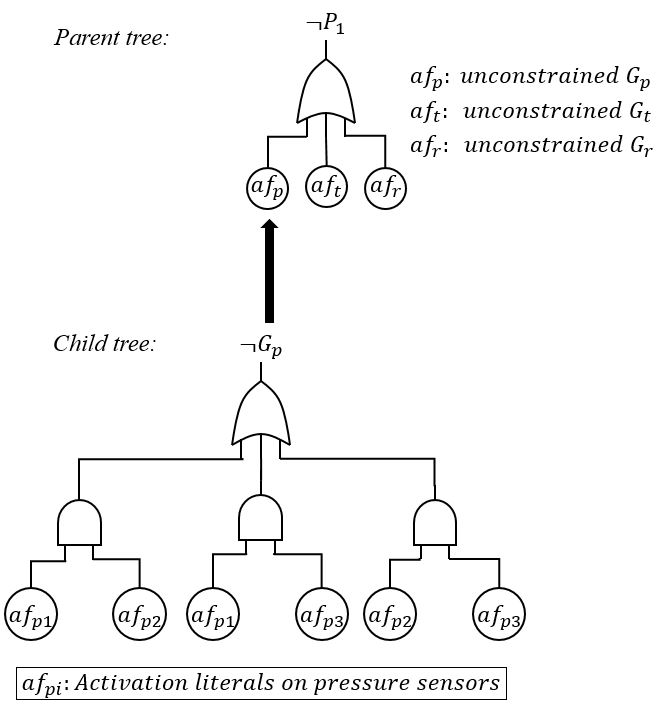
\includegraphics[width=0.5\textwidth]{images/faultCompEx.JPG}
	\end{center}
	\caption{Sensor System Composition of Fault Trees}
	\label{fig:sensorSysComp}
\end{figure}
We return to the sensor system example to illustrate this mapping. Graphically, this is represented in Figure~\ref{fig:sensorSysComp}.  The top level (parent) component is defined as: $\mathit{Comp}_p (M_p, \mathit{FF}_p, \mathit{NFV}_p, \pi_p)$ and $\mathit{FF}_p = \{(\neg P, \mathit{af}_p \lor \mathit{af}_t \lor \mathit{af}_r)\}$ where each activation literal is associated with the unconstrained guarantees $G_p$, $G_t$, and $G_r$. The child layer has a fault forest consisting of three fault trees, one for each subsystem. 

The pressure subsystem fault tree is $\mathit{FT}_{p} = (\neg G_p, (\mathit{af}_{p1} \land \mathit{af}_{p2}) \lor (\mathit{af}_{p1} \land \mathit{af}_{p3}) \lor (\mathit{af}_{p2} \land \mathit{af}_{p3}) $. The leaf formulae for each subsystem tree corresponds to pairwise combinations of active sensor faults. We now show the composition of the pressure subsystem child and top level parent fault trees. 

The mapping $\phi_F$ iterates through each tree in the parent forest -- in this case, we have only one. Then for each parent tree it iterates through the Boolean literals in $\mathcal{L}$. If there is a match between a child root and a parent leaf, the replacement is made. We represent the unconstrained (violated) guarantee as $\neg G_p$ and it is associated with the fault activation literal $\mathit{af}_p$. Thus, $\mathit{af}_p$ will be extended with $\{\neg G_p, (\mathit{af}_{p1} \land \mathit{af}_{p2}) \lor (\mathit{af}_{p1} \land \mathit{af}_{p3}) \lor (\mathit{af}_{p2} \land \mathit{af}_{p3})\}$. This extension is done for each leaf formula in $\mathcal{L}_p$ from the parent fault forest. The end result of the replacement is easy to see in Figure~\ref{fig:sensorSysComp}.

%%%%5										COMPOSITION OF FF IS VALID
\begin{lemma} If $\mathit{FF_c}$ and $\mathit{FF_p}$ are valid fault forests, then their composition $\phi(\mathit{FF_c}, \mathit{FF_p})$ is also a valid fault forest. 
\begin{proof}

Assume the antecedent. Then for all $\mathit{FT_j} \in \mathit{FF_p}$ and $\mathit{FT_i} \in \mathit{FF_c}$, $\mathit{FT_i}$ and $\mathit{FT_j}$ are valid fault trees as per Definition~\ref{def:validFF}. For each iteration defined in the mapping $\phi_F$, apply Lemma~\ref{lemma:validTree} and the monotonicity assumption. 

\end{proof}
\label{lemma:validForest}
\end{lemma}











%%				DEFINE COMPOSITION OF COMPONENTS
We have provided the foundational definitions necessary to discuss what it means to compose components. The composition of child component $\mathit{Comp}_c$ and parent component $\mathit{Comp}_p$ is defined as:

\begin{definition}
$Comp_c(M_c, \mathit{FF}_c, \mathit{NFV}_c, \pi_c) \circ Comp_p(M_p, \mathit{FT}_p, \mathit{NFV}_p, \pi_p) $\\$= Comp_\circ(M', \mathit{FF}', \mathit{NFV}', \pi')$ where:
\begin{itemize}[label=\textbullet]
\item $M' = M_c \cup M_p$ is the iterative enlargement of the model by combining children guarantees with parent guarantees,
\item $\mathit{FF}_c \circ \mathit{FF}_p$ is the composed fault forest
\item $\mathit{NFV}' = \mathit{NFV}_c \cup \mathit{NFV}_p$ is the set of non-faulty variables
\item $\pi' = \pi_c \cup \pi_p$ are valid properties such that $(I, T'(\mathit{NFV}')) \vdash \pi'$.
\end{itemize}
\end{definition}

The enlargement of the model, $M'$, iteratively flattens the composed layers by taking the union of children guarantees and parent guarantees. The fault forests are composed into a set of fault trees describing the enlarged model. The non-faulty variables from child and parent are combined into a set $\mathit{NFV'}$ such that $(I, T'(\mathit{NFV}')) \vdash \pi'$. 


%%				NFV |- PI
Given that in child and parent components, the properties $\pi$ can be derived from the non-faulty variables, we show that this relationship holds after composition. To state $(I, T'(\mathit{NFV})) \vdash \pi$, we use the shorthand $\mathit{NFV} \vdash \pi$. 

\begin{theorem} If $\mathit{NFV}_c \vdash \pi_c$ and $\mathit{NFV}_p \vdash \pi_p$, then $\mathit{NFV}' \vdash \pi'$
\begin{proof}
Assume antecedent. Let $p' \in \pi'$. If $p' \in \pi_c$ then $\mathit{NFV}_c \vdash p'$ and likewise if $p' \in \pi_p$, then $\mathit{NFV}_p \vdash p'$. In either case, $\mathit{NFV}_c \cup \mathit{NFV}_p = \mathit{NFV}' \vdash \pi'$.
\end{proof}
\end{theorem} 


We have shown that a single layer of composition produces valid fault forests. To perform this analysis across $n$ layers of architecture we use induction to show that the resulting fault forest is valid. 

The notation $\phi_F^n$ indicates the iterated function $\phi_F$ which is a successive application of $\phi_F$ with itself $n$ times. Assume the fault forest $\mathit{FF_0}$ is obtained at the leaf level of the architecture.

\begin{theorem} If $\phi_F^n(\mathit{FF_{n-1}}, \mathit{FF_n})$ is a valid fault forest, then $\phi^{n+1}(\mathit{FF_n}, \mathit{FF_{n+1}})$ is a valid fault forest.
\begin{proof}

Base case: Each fault forest per layer is valid by construction. By Lemma~\ref{lemma:validForest}, $\phi_F(\mathit{FF_0}, \mathit{FF_1})$ is a valid fault forest.

Inductive assumption: Assume $\phi_F^n(\mathit{FF_{n-1}}, \mathit{FF_n})$ is a valid fault forest.
\begin{equation*}
\begin{split}
\phi_F^{n+1}(\mathit{FF_n}, \mathit{FF_{n+1}}) &= ((\mathit{FF_0} \circ \mathit{FF_1}) \circ \mathit{FF}_2) \circ \cdots \circ \mathit{FF_n}) \circ \mathit{FF_{n+1}})) \\
  &= \phi_F^n(\mathit{FF_{n-1}}, \mathit{FF_n}) \circ \mathit{FF_{n+1}}
\end{split}
\end{equation*}

%$\phi_F^{n+1}(\mathit{FF_n}, \mathit{FF_{n+1}}) = ((\mathit{FF_0} \circ \mathit{FF_1}) \circ \mathit{FF}_2) \circ \cdots \circ \mathit{FF_n}) \circ \mathit{FF_{n+1}})) = \phi_F^n(\mathit{FF_{n-1}}, \mathit{FF_n}) \circ \mathit{FF_{n+1}}$. 

By inductive assumption and Lemma~\ref{lemma:validForest}, $\phi_F^{n+1}(\mathit{FF_n}, \mathit{FF_{n+1}})$ is a valid fault forest.

\end{proof}
\label{thm:indForest}
\end{theorem}

\begin{comment}
We know from previous work that composition is conservative. A valid monolithic analysis of the transition system implies that the compositional analysis of that same system is valid, but the converse may not be true~\cite{}. It is likewise the case for composing fault forests. 

Let $S \subseteq \mathit{AF}$ where all $\mathit{af} \in S$ are constrained to true. If $S \cup \{\neg P\}$ is satisfiable, this equates to a valid fault tree. 

\begin{theorem} If $(I,T) \vdash P$ for monolithic verification, then for $S \subseteq \mathit{AF}$, $S \cup \{\neg P\}$ is unsatisfiable.
\begin{proof}
Assume toward contradiction that $(I,T) \vdash P$ and there exists a set $S \subseteq \mathit{AF}$ such that $S \cup \{\neg P\}$ is satisfiable. This implies that there exists a reachable state such that $\neg P$ holds. This contradicts our assumption. 
\end{proof}
\label{thm:sound}
\end{theorem}

As a counterexample to the converse of Theorem~\ref{thm:sound}, consider the following. \danielle{Counterexample here.}

\end{comment}

In this section, we have formalized the idea that fault trees (and forests) can be composed without losing the validity of each composed tree. We proved that this can be performed iteratively across an arbitrary number of layers. Now that we have the formal foundations laid, we proceed towards the implementation. 


